\section{Design Language}
\label{design:design_language}
As stated, the design language is a collection of design standards, specifically for the \giraf[] system. 
The design language is based on usability concerns found in \autoref{Preanalysis:Usability_for_children}.

\subsection{Status icons}
\label{design:state_icons}

In the \giraf[] system there are different status icons for showing the user what an action will do or is doing. All these icons can be seen in \autoref{fig:status_icons}. If an action accepts, the leftmost icon will be used and if a window is loading, the fourth leftmost icon will be shown so the user knows the system is loading.

\begin{figure}[h!]
	\centering
	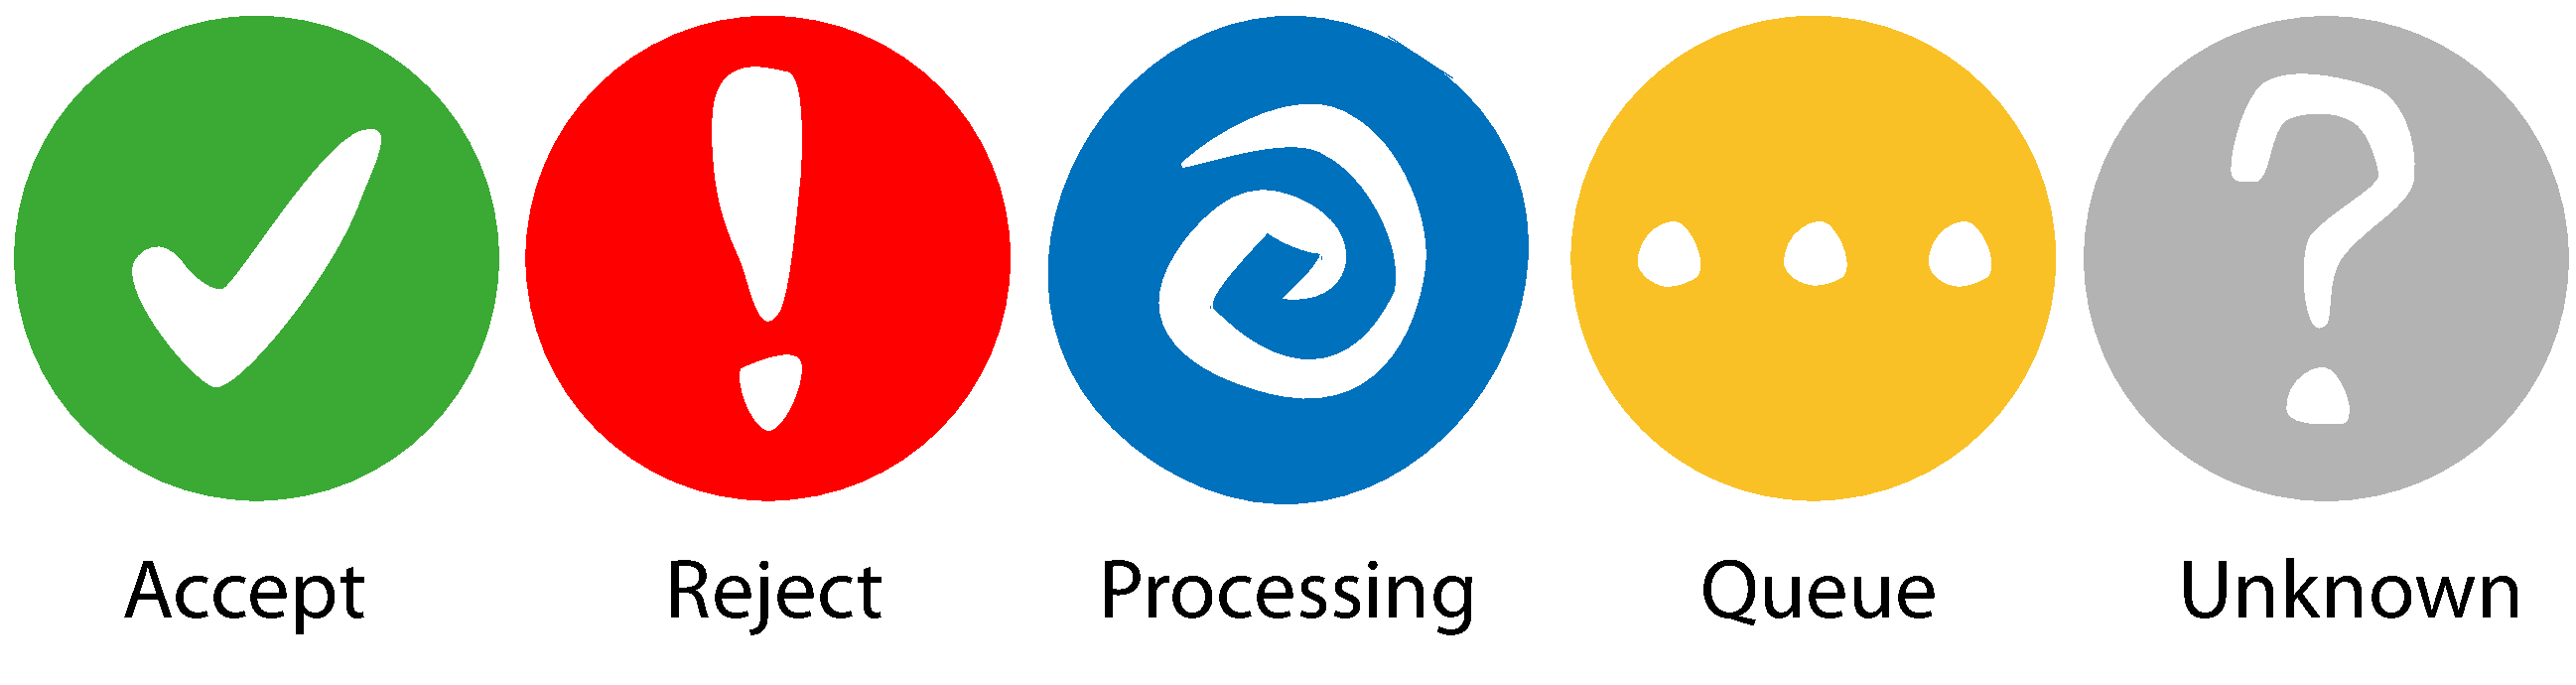
\includegraphics[width=\textwidth]{gfx/status_icons}
	\caption{Status icons in the \giraf[] system}
	\label{fig:status_icons}
\end{figure}

\subsection{Colors}
\label{design:giraf_colors}

Colors where chosen for the \giraf[] system, these can be seen in \autoref{fig:colortheme}. These colors are designed for use in two different cases. The first four yellow and brown colors are chosen for use together, and the last four colors, white and grey, are made for use together. 
These color groups were chosen, such that they contained colors with contrast, and colors that could be used for gradients.

\begin{figure}[h!]
	\centering
	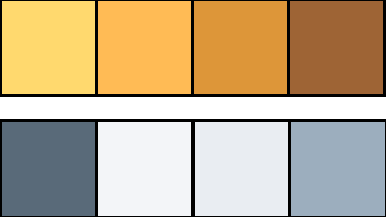
\includegraphics[width=0.5\textwidth]{gfx/design_color_theme}
	\caption{The color theme of the \giraf[] system}
	\label{fig:colortheme}
\end{figure}

\begin{figure}[h!]
	\centering
	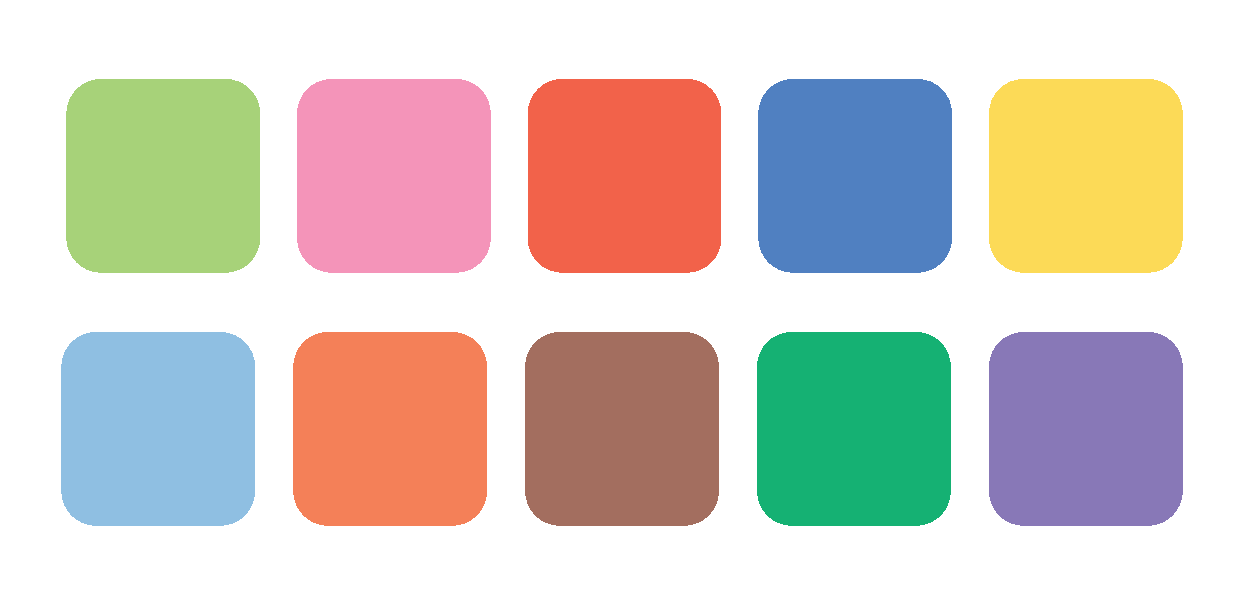
\includegraphics[width=0.5\textwidth]{gfx/app_colors.pdf}
	\caption{App colors of the \giraf[] system}
	\label{fig:appcolors}
\end{figure}

The colors shown in \autoref{fig:appcolors}, are the app colors available in the \giraf[] system.
These colors are chosen to be dark, to allow white silhouettes to be placed on top of them, while letting the silhouettes remain clearly visible.

\subsection{Interactive elements}
\label{design:button_design}

The idea is for all interactive elements in the \giraf[] system to have round corners, and if an element is not interactive, it should have square corners.

An example can be seen in \autoref{fig:buttons}, where two button illustrations are shown, but the system also includes draggable objects and other interactive objects.

\begin{figure}[h!]
	\centering
	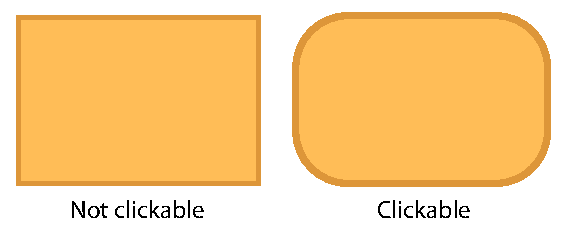
\includegraphics[width=0.4\textwidth]{gfx/buttons.pdf}
	\caption{Interactive elements: Buttons illustrations}
	\label{fig:buttons}
\end{figure}